\chapter{Calcul Stochastique}

\section{Temps d'arrêt}

\subsection*{Exercice :}

\begin{exerciseBox}[Temps d'arrêt]
Deux joueurs, A et B, s'affrontent à un jeu de pile ou face.  
\begin{itemize}
    \item Le joueur A commence avec $a$ jetons,  
    \item  Le joueur B avec $b$ jetons.  
\end{itemize}

à chaque tour, on lance une pièce équitable :  
\begin{itemize}
    \item  Si A gagne, il prend un jeton à B,  
    \item Sinon, il en perd un au profit de B.  
\end{itemize}

Le jeu continue jusqu’à ce que l’un des deux joueurs ait tous les jetons.  
Quelle est la probabilité que A gagne la partie ?    
\end{exerciseBox}

\subsection*{Solution :}

Soit $(\epsilon_n)_{n \geq 1}$ une suite de variables aléatoires i.i.d. définies par :
\[
\mathbb{P}(\epsilon_n = +1) = \mathbb{P}(\epsilon_n = -1) = \frac{1}{2}.
\]

Définissons $(X_n)$, le nombre de jetons du joueur A après $n$ tours :
\[
X_n = a + \sum_{i=1}^n \epsilon_i, \quad \text{avec } X_0 = a.
\]

Soit $\tau$ le \textbf{temps d'arrêt} correspondant à la fin de la partie :
\[
\tau := \inf \{ n \geq 0 \mid X_n = 0 \text{ ou } X_n = a + b \}.
\]

C’est le premier instant où A ou B perd tous ses jetons.

\vspace{0.5cm}

On a :
\begin{itemize}
    \item  \textbf{martingale} par rapport à la filtration naturelle $(\mathcal{F}_n)$.
    
    \item  $\tau$ est un \textbf{temps d'arrêt} (car $X_n$ est adapté, et $\{ \tau \leq n \} \in \mathcal{F}_n$).
    
    \item De plus, $\tau$ est \textbf{presque sûrement fini} (le processus atteint presque sûrement l’un des bords).

\end{itemize}


Par le \textbf{théorème du temps d'arrêt}, si $(X_n)$ est une martingale et $\tau$ est un temps d'arrêt presque sûrement fini, alors :
\[
\mathbb{E}[X_\tau] = \mathbb{E}[X_0] = a.
\]


Or $X_\tau$ ne prend que les valeurs $0$ (si B gagne) ou $a + b$ (si A gagne), donc :
\[
\mathbb{E}[X_\tau] = 0 \cdot \mathbb{P}(A \text{ perd}) + (a + b) \cdot \mathbb{P}(A \text{ gagne}) = (a + b) \cdot \mathbb{P}(A > B).
\]

D’où :
\[
\boxed{\mathbb{P}(A > B) = \frac{a}{a + b}}.
\]
% or $X_\tau \in {0 , a+b}$ avec la proba  $p := \mathbb{P}(A \text{ gagne}) = \mathbb{P}(X_\tau = a + b)$ , donc 

% % \paragraph{Loi de $X_\tau$.}

% % Le processus s’arrête dès que $X_n$ atteint $0$ ou $a + b$. Donc $X_\tau$ prend uniquement deux valeurs possibles :
% % \begin{itemize}
% %     \item  $X_\tau = 0$ (A a tout perdu),
% %     \item $X_\tau = a + b$ (A a tout gagné).
% % \end{itemize}

% % Soit $p := \mathbb{P}(A \text{ gagne}) = \mathbb{P}(X_\tau = a + b)$.

% Alors :
% \[
% \mathbb{E}[X_\tau] = 0 \cdot \mathbb{P}(X_\tau = 0) + (a + b) \cdot \mathbb{P}(X_\tau = a + b) = (a + b) \cdot p.
% \]

% On a aussi $\mathbb{E}[X_\tau] = a$ d'après l’étape précédente, donc :
% \[
% a = (a + b) \cdot p \quad \Rightarrow \quad p = \frac{a}{a + b}.
% \]

% \paragraph{Conclusion :}

% La probabilité que A gagne contre B est :
% \[
% \boxed{\mathbb{P}(A > B) = \frac{a}{a + b}}.
% \]

\paragraph{Preuve que  $\tau < \infty$ p.s.}

Il s'agit de montrer que :
\[
\mathbb{P}(\tau <  +\infty) = 1 \quad \Longleftrightarrow \quad \mathbb{P}(\tau = +\infty) = 0  \Longleftrightarrow \quad \lim_{n \to \infty} \mathbb{P}(\tau > n) = 0 
\]

Soit \( n \in \mathbb{N} \). On a :
\[
\tau > n \quad \Longleftrightarrow \quad 0 < X_k < a + b \quad \text{pour tout } k \leq n.
\]

En particulier :
\[
\tau > n \quad \Longrightarrow \quad 0 < X_n = a + \sum_{i=1}^n \epsilon_i < a + b.
\]

Ce qui revient à :
\[
-a < \sum_{i=1}^n \epsilon_i < b \quad \Longleftrightarrow \quad \frac{-a}{\sqrt{n}} < \frac{1}{\sqrt{n}} \sum_{i=1}^n \epsilon_i < \frac{b}{\sqrt{n}}.
\]

Donc :
\[
\mathbb{P}(\tau > n) = \mathbb{P}\left( \frac{-a}{\sqrt{n}} < \frac{1}{\sqrt{n}} \sum_{i=1}^n \epsilon_i < \frac{b}{\sqrt{n}} \right) =  \mathcal{E}_n\left( \frac{b}{\sqrt{n}} \right) - \mathcal{E}_n\left( \frac{-a}{\sqrt{n}} \right),
\]
où \( \mathcal{E}_n \) est la fonction de répartition de \( \frac{1}{\sqrt{n}} \sum_{i=1}^n \epsilon_i \).

Or lorsque \( n \to \infty \), on a :
\[
\frac{1}{\sqrt{n}} \sum_{i=1}^n \epsilon_i \xrightarrow{d} \mathcal{N}(0,1),
\]
donc :
\[
\mathcal{E}_n \xrightarrow[n \to \infty]{} \Phi \quad \text{où } \Phi \text{ est la f.d.r. de } \mathcal{N}(0,1).
\]

Ainsi :
\[
\lim_{n \to \infty} \mathbb{P}(\tau > n) = \int_{-a/\sqrt{n}}^{b/\sqrt{n}} f_{\mathcal{E}_n}(x) \, dx \xrightarrow[n \to \infty]{} \int_{0}^{0} f(x) \, dx = 0.
\]

Donc :
\[
\boxed{\mathbb{P}(\tau = +\infty) = 0}.
\]


\section{Loi de l'intégrale du mouvement brownien}

\subsection*{Exercice :}

\begin{exerciseBox}[Loi de l'intégrale du mouvement brownien]
Soit \( (W_t)_{t \geq 0} \) un mouvement brownien standard, et soit :
\[
X := \int_0^T W_t \, dt
\]

\textbf{Question :} Déterminer la loi de \( X \) (loi exacte : nature, espérance, variance).
\end{exerciseBox}


\subsection*{Solution :}


Soit \( (W_t)_{t \geq 0} \) un mouvement brownien standard. On pose :
\[
X := \int_0^T W_t \, dt
\]

On considère la fonction :
\[
f(t, x) = tx
\]

On applique la formule d'Itô sur \( f(t, W_t) \) :

\[
df(t, W_t) = \frac{\partial f}{\partial t} dt + \frac{\partial f}{\partial x} dW_t + \frac{1}{2} \frac{\partial^2 f}{\partial x^2} dt
\]

\[
\frac{\partial f}{\partial t} = W_t,\quad
\frac{\partial f}{\partial x} = t,\quad
\frac{\partial^2 f}{\partial x^2} = 0
\]

\[
\Rightarrow d(t W_t) = W_t dt + t dW_t
\]

Intégration entre 0 et \( T \) :

\[
\int_0^T W_t \, dt = T W_T - \int_0^T t \, dW_t
\quad \Rightarrow \quad
X = T W_T - \int_0^T t \, dW_t
\]

donc 

\[
\boxed{
\int_0^T W_t \, dt = \int_0^T (T - t) \, dW_t
}\]



\begin{rappelBox}[loi de l'intégrale de Wiener]
Soit \( f \in L^2([0,T]) \) déterministe, alors :
\[
\int_0^T f(t) \, dW_t \sim \mathcal{N}\left(0, \int_0^T f^2(t)\, dt\right)
\]
\end{rappelBox}



\subsection*{Application à \( X = \int_0^T W_t\, dt \)}

On a :
\[
X = \int_0^T W_t \, dt = \int_0^T (T - t) \, dW_t
\]



\[
\mathbb{E}[X]  = 0
\]

\[
\operatorname{Var}(X) = \int_0^T (T-t)^2dt = \frac{T^3}{3}
\]



\subsection*{Conclusion}

\[
\boxed{
\int_0^T W_t \, dt \sim \mathcal{N}\left(0,\ \frac{T^3}{3} \right)
}
\]

\vspace{1cm}


\section{Espérance conditionnelle d'un mouvement brownien}

\subsection*{Exercice :}

\begin{exerciseBox}[Espérance conditionnelle d'un mouvement brownien]
Soit \( (W_t)_{t \geq 0} \) un mouvement brownien standard.

\vspace{1cm}

\textbf{Question :} Calculer \( \mathbb{E}[W_t \mid W_s] \)
\end{exerciseBox}

\subsection*{Solution :}

Soit \( (W_t)_{t \geq 0} \) un mouvement brownien standard. On considère deux cas selon les positions relatives de \( t \) et \( s \), tous deux strictement positifs.

\subsection*{Cas 1 : \( t > s \)}

Par propriété de martingale (adaptation naturelle), on a :

\[
\mathbb{E}[W_t \mid \mathcal{F}_s] = W_s
\Rightarrow
\mathbb{E}[W_t \mid W_s] = \mathbb{E}\left[\mathbb{E}[W_t \mid \mathcal{F}_s] \mid W_s\right] = W_s
\]

\[
\boxed{
\mathbb{E}[W_t \mid W_s] = W_s \quad \text{si } t > s
}
\]


\subsection*{Cas 2 : \( 0 < t < s \)}

\begin{rappelBox}
Soient \( 0 < u < v \), le \textbf{pont brownien} de \( u \) à \( v \) est défini par :
\[
B_t^{u,v} := W_t - \frac{t - u}{v - u}(W_v - W_u), \quad t \in [u, v]
\]

Alors :
\begin{itemize}
  \item \( (B_t^{u,v})_t \) est un processus continu, centrée gaussien
  \item $(B_t^{u,v})_t$ indépendants de $\sigma(W_s , s \leq u)$ et $\sigma(W_s , s \geq v)$ 
\end{itemize}
\end{rappelBox}

Application à notre cas \( 0 < t < s \) :

\[
W_t = \left(W_t - \frac{t}{s}W_s\right) + \frac{t}{s}W_s
\]

\[
\text{On note } \widehat{W}_t := W_t - \frac{t}{s} W_s \quad \Rightarrow \quad
W_t = \widehat{W}_t + \frac{t}{s} W_s
\]

\[
\text{Or } \widehat{W}_t \perp W_s \quad \Rightarrow \quad \mathbb{E}[\widehat{W}_t \mid W_s] = 0
\]

Donc :
\[
\mathbb{E}[W_t \mid W_s] = \mathbb{E}\left[\widehat{W}_t + \frac{t}{s} W_s \mid W_s \right]
= \frac{t}{s} W_s
\]

\[
\boxed{
\mathbb{E}[W_t \mid W_s] = \frac{t}{s} W_s \quad \text{si } 0 < t < s
}
\]




\subsection*{Conclusion}

\[
\boxed{
\mathbb{E}[W_t \mid W_s] =
\begin{cases}
W_s & \text{si } t > s \\
\frac{t}{s} W_s & \text{si } t < s
\end{cases}
}
\]



\section{Espérance conditionnelle d'une intégrale stochastique}

\subsection*{Exercice :}

\begin{exerciseBox}[Espérance conditionnelle d'une intégrale stochastique]
Soit $(B_s)_{s \geq 0}$ M.B.S et $t \in \mathbb{R}^+$

\textbf{Question :} calculer 
$$
\mathbb{E}\left[ \int_0^t s dB_s \mid B_t  \right] 
$$
\end{exerciseBox}


\subsection*{Solution :}

On pose :
\[
\Phi(b) := \mathbb{E} \left[ \int_0^t s\, dB_s \,\middle|\, B_t = b \right]
\]

\subsection*{Étape 1 : Formule d'Itô}

On applique Itô à la fonction \( f(s, B_s) = s B_s \) :

\[
d(s B_s) = B_s\, ds + s\, dB_s
\quad \Rightarrow \quad
s\, dB_s = d(s B_s) - B_s\, ds
\]

On intègre entre 0 et \( t \) :

\[
\int_0^t s\, dB_s = t B_t - \int_0^t B_s\, ds
\]


\subsection*{Étape 2 : Espérance conditionnelle}

On remplace dans \( \Phi(b) \) :

\[
\Phi(b) = \mathbb{E} \left[ t B_t - \int_0^t B_s\, ds \,\middle|\, B_t = b \right]
= t b - \mathbb{E} \left[ \int_0^t B_s\, ds \,\middle|\, B_t = b \right]
\]


\subsection*{Étape 3 : Fubini}

Comme \( B_s \) est uniformément intégrable, on peut échanger intégrale et espérance :

\[
\Phi(b) = t b - \int_0^t \mathbb{E}[B_s \mid B_t = b]\, ds
\]


\subsection*{Étape 4 : Pont brownien}

Pour \( 0 \leq s \leq t \), par la propriété du pont brownien :

\[
\mathbb{E}[B_s \mid B_t = b] = \frac{s}{t} b
\]

Donc :
\[
\Phi(b) = t b - \int_0^t \frac{s}{t} b\, ds = t b - \frac{b}{t} \int_0^t s\, ds
= t b - \frac{b}{t} \cdot \frac{t^2}{2} = t b - \frac{t}{2} b = \frac{t}{2} b
\]


\subsection*{Conclusion}

\[
\mathbb{E} \left[ \int_0^t s\, dB_s \,\middle|\, B_t \right] = \frac{t}{2} B_t
\quad \Rightarrow \quad
\boxed{
\mathbb{E} \left[ \int_0^t s\, dB_s \,\middle|\, B_t \right] = \frac{t}{2} B_t
}
\]


\section{MBG}

\subsection*{Exercice :}

\begin{exerciseBox}[MBG]
Soit \( (W_t)_{t \geq 0} \) un mouvement brownien standard, et soit \( S_t \) un processus satisfaisant l'équation différentielle stochastique suivante :
\[
dS_t = \mu S_t\, dt + \sigma S_t\, dW_t, \quad S_0 > 0
\]

\textbf{Question :} Déterminer une expression explicite de \( S_t \).
\end{exerciseBox}


\subsection*{Solution :}

On souhaite résoudre l'équation stochastique :
\[
dS_t = \mu S_t\, dt + \sigma S_t\, dW_t, \quad S_0 > 0
\]


\subsection*{Étape 1 : Changement de variable \( Y_t := \log S_t \)}

On applique le lemme d'Itô à la fonction \( f(x) = \log x \), avec \( S_t > 0 \) :

\[
dY_t = d(\log S_t) = \frac{1}{S_t} dS_t - \frac{1}{2} \frac{1}{S_t^2} (dS_t)^2
\]

\[
= \frac{1}{S_t} (\mu S_t\, dt + \sigma S_t\, dW_t) - \frac{1}{2} \frac{1}{S_t^2} \sigma^2 S_t^2\, dt
\]

\[
= \mu\, dt + \sigma\, dW_t - \frac{1}{2} \sigma^2\, dt
\quad \Rightarrow \quad
dY_t = \left(\mu - \frac{\sigma^2}{2} \right) dt + \sigma\, dW_t
\]


\subsection*{Étape 2 : Intégration de \( Y_t \)}

\[
Y_t = \log S_t = \log S_0 + \left(\mu - \frac{\sigma^2}{2} \right)t + \sigma W_t
\]


\subsection*{Étape 3 : Retour à \( S_t \)}

\[
S_t = \exp(Y_t) = S_0 \cdot \exp\left( \left(\mu - \frac{\sigma^2}{2} \right)t + \sigma W_t \right)
\]


\subsection*{Conclusion}

\[
\boxed{
S_t = S_0 \cdot \exp\left( \left(\mu - \frac{\sigma^2}{2} \right)t + \sigma W_t \right)
}
\]


\section{Processus d'Ornstein-Uhlenbeck}

\subsection*{Exercice :}

\begin{exerciseBox}[Processus d'Ornstein-Uhlenbeck]
Soit \( (W_t)_{t \geq 0} \) un mouvement brownien standard. On considère le processus \( X_t \) solution de l’équation différentielle stochastique suivante :
\[
dX_t = -a X_t\, dt + \sigma\, dW_t, \quad X_0 = x_0, \quad a > 0, \; \sigma > 0
\]

\textbf{Question :} Déterminer la loi  de \( X_t \).
\end{exerciseBox}

\subsection*{Solution :}

On pose le facteur intégrant :
\[
Y_t := e^{a t} X_t
\]

Par la formule d’Itô pour \( f(t, X_t) = e^{a t} X_t \), on a :
\[
dY_t = \frac{\partial f}{\partial t}\, dt + \frac{\partial f}{\partial x}\, dX_t = a e^{a t} X_t\, dt + e^{a t} \, dX_t
\]

En remplaçant \( dX_t \) dans cette expression :
\[
dY_t = a e^{a t} X_t\, dt + e^{a t} (-a X_t\, dt + \sigma\, dW_t) = a e^{a t} X_t\, dt - a e^{a t} X_t\, dt + \sigma e^{a t} \, dW_t
\]

\[
\Rightarrow dY_t = \sigma e^{a t} dW_t
\]

En intégrant des deux côtés de \( 0 \) à \( t \) :
\[
Y_t = Y_0 + \int_0^t \sigma e^{a s} dW_s = x_0 + \sigma \int_0^t e^{a s} dW_s
\]

Donc :
\[
X_t = e^{-a t} Y_t = x_0 e^{-a t} + \sigma e^{-a t} \int_0^t e^{a s} dW_s
\]

\[
\boxed{
X_t = x_0 e^{-a t} + \int_0^t \sigma e^{-a(t-s)} dW_s
}
\]




\vspace{0.2cm}
\textbf{Espérance :}
\[
\mathbb{E}[X_t] = x_0 e^{-a t}
\]

\textbf{Variance :}
\[
\operatorname{Var}(X_t) = \sigma^2 e^{-2a t} \int_0^t e^{2a s} ds = \sigma^2 \cdot \frac{1 - e^{-2a t}}{2a}
\]

\vspace{0.3cm}
Donc : 

\[
\boxed{
X_t \sim \mathcal{N} \left( x_0 e^{-a t}, \; \frac{\sigma^2}{2a} \left( 1 - e^{-2a t} \right) \right)
}
\]

\[
\boxed{
X_t \sim_{t \rightarrow +\infty} \mathcal{N} \left( 0, \; \frac{\sigma^2}{2a}) \right)
}
\]


\section{Probabilité de sortie à gauche d’un intervalle – O.U.}

\subsection*{Exercice :}

\begin{exerciseBox}[Probabilité de sortie à gauche d’un intervalle – O.U.]
Soit \( (W_t)_{t \geq 0} \) un mouvement brownien standard, et soit \( X_t \) défini par :
\[
dX_t = -a X_t\, dt + \sigma\, dW_t, \quad X_0 = x \in (b, c), \quad \text{avec } a > 0, \; \sigma > 0 ,\; \; b \leq 0 \leq c 
\]

On définit le temps d’arrêt :
\[
T := \inf\{t \geq 0 \;|\; X_t \notin (b, c)\}
\]

 On admettra que $\mathbb{P}(T < \infty) = 1$.

\textbf{Question :} Déterminer la probabilité que \( X_t \) sorte par le bas, c’est-à-dire :
\[
\mathbb{P}(X_T = b)
\]
\end{exerciseBox}

\subsection*{Solution :}

L’idée est de construire une fonction $f$ telle que $(f(X_t))_{t\ge 0}$ soit une martingale.  
On pourra alors appliquer le théorème de temps arrêt pour calculer $\mathbb{E}[f(X_T)]$ , et en déduire $\mathbb{P}(X_T=b)$.

\medskip
\textbf{Étape 1 – Recherche de $f$}\\
On cherche $f\in \mathcal{C}^2$ vérifiant que $f(X_t)$ est une martingale.  
En appliquant la formule d’Itô à $f(X_t)$ :
\[
df(X_t)=f'(X_t)dX_t+\tfrac{1}{2}f''(X_t)\sigma^2 dt
      =\Big[-aX_t f'(X_t)+\tfrac{\sigma^2}{2}f''(X_t)\Big]dt
       +\sigma f'(X_t)dW_t.
\]
Pour annuler le terme en $dt$, $f$ doit donc satisfaire l’équation différentielle
\[
\frac{\sigma^2}{2}f''(x)-a x f'(x)=0. \quad f(0) = 0 , f'(0) = 1
\]
On pose $g(x)=f'(x)$, ce qui conduit à
\[
g'(x)-\frac{2a}{\sigma^2}x g(x)=0
\quad\Longrightarrow\quad
g(x)=\lambda \exp\!\Big(\tfrac{a}{\sigma^2}x^2\Big).
\]
En intégrant et en choisissant $f(0)=0$ (constante arbitraire), on obtient
\[
f(x)=\lambda \int_0^x \exp\!\Big(\tfrac{a}{\sigma^2} y^2\Big)dy.
\]
comme $f'(0) = 1$ donc $\lambda=1$

% On peut normaliser $\lambda=1$ car elle s’éliminera dans le rapport final.

\medskip
\textbf{Étape 2 – Théorème d’arrêt}\\

Soit $n \in \mathbb{N}$.  
Comme $(f(X_t))_{t\geq 0}$ est une martingale et que $T_n := T \wedge n$ est un temps d'arrêt borné, le théorème d’arrêt donne
\[
\mathbb{E}\big[f(X_{T_n})\big] = \mathbb{E}[f(X_0)] = 0.
\]

Pour pouvoir échanger la limite et l’espérance, c’est-à-dire écrire
\[
\lim_{n \to +\infty} \, \mathbb{E}\big[f(X_{T_n})\big] 
= \mathbb{E}\!\left(\lim_{n \to +\infty} f(X_{T_n})\right),
\]
il faut appliquer le théorème de la convergence dominée.

\begin{itemize}
  \item Lorsque $n \to +\infty$, on a $T_n = T \wedge n \to T$ presque sûrement.
  \item De plus, $|f(X_{T_n})| \leq \sup_{|t|\leq n} |f(X_t)|$, et comme $n$ est fini, cette borne est intégrable.
\end{itemize}

Ainsi, par le théorème de la convergence dominée , on obtient
\[
\mathbb{E}[f(X_T)] = \mathbb{E}[f(X_0)] = 0.
\]



Or $X_T\in\{b,c\}$, donc
\[
\mathbb{E}\big[f(X_T)\big]=f(b)\,\mathbb{P}(X_T=b)+f(c)\,\mathbb{P}(X_T=c)
     =f(b)\,\mathbb{P}(X_T=b)+f(c)\bigl[1-\mathbb{P}(X_T=b)\bigr].
\]
Il en résulte
\[
\mathbb{P}(X_T=b)
= \frac{f(c)}{f(c)-f(b)}
= \frac{\displaystyle\int_0^c \exp\!\bigl(\tfrac{a}{\sigma^2} y^2\bigr)dy}
       {\displaystyle\int_b^c \exp\!\bigl(\tfrac{a}{\sigma^2} y^2\bigr)dy}.
\]

\medskip
\textbf{Réponse finale :}
\[
\boxed{\;
\mathbb{P}(X_T = b)
= \frac{\displaystyle\int_0^{c} e^{\frac{a}{\sigma^{2}} y^{2}}\,dy}
       {\displaystyle\int_{b}^{c} e^{\frac{a}{\sigma^{2}} y^{2}}\,dy}
\;}
\]


\section{Hitting time of brownian motion}

\subsection*{Exercice :}

\begin{exerciseBox}[Hitting Time of Brownian Motion]
Let \( (W_t)_{t \ge 0} \) be a standard Brownian motion and define the \textbf{hitting time} of level \( a \in \mathbb{R} \) by:
\[
\tau_a := \inf\{\, t \ge 0 \mid W_t = a \,\}.
\]

\textbf{Questions:}
\begin{enumerate}
  \item Show that $\forall a \in \mathbb{R}, \forall u \in \mathbb{R}^{+}$ :
    \[
    M_{\tau_a}(u) := \mathbb{E}\big[e^{-u \tau_a}\big] = e^{-|a| \sqrt{2u}}.
    \]
  \item Show that \( \tau_a < +\infty \) almost surely, and that \( \mathbb{E}[\tau_a] = +\infty. \)   
\end{enumerate}
\end{exerciseBox}

\subsection*{Solution :}


\textbf{Step 1 – Trivial case.}  
If \( a = 0 \), then by definition \( \tau_0 = 0 \) and \( M_{\tau_0}(u) = 1 = e^{-|a|\sqrt{2u}} \).  
Hence, the formula holds.

\medskip
\textbf{Step 2 – Case \( a > 0 \).}  
Consider the exponential martingale:
\[
N_t := \exp\!\left( \sigma W_t - \frac{\sigma^2 t}{2} \right), \qquad \sigma > 0.
\]
Since \( (N_t)_{t \ge 0} \) is a positive martingale, by the \textbf{optional stopping theorem} applied to the bounded stopping time \( \tau_a \wedge t \), we have:
\[
\mathbb{E}[N_{\tau_a \wedge t}] = \mathbb{E}[N_0] = 1.
\]

\medskip
\textbf{Decomposition:}
\[
\mathbb{E}[N_{\tau_a \wedge t}]
= \mathbb{E}\!\left[N_{\tau_a}\mathbf{1}_{\{\tau_a < t\}}\right]
+ \mathbb{E}\!\left[N_t \mathbf{1}_{\{\tau_a \ge t\}}\right].
\]

As \( N_t \ge 0 \), monotone convergence gives:
\[
\lim_{t \to \infty} \mathbb{E}\!\left[N_{\tau_a \wedge t}\right]
= \mathbb{E}\!\left[N_{\tau_a} \mathbf{1}_{\{\tau_a < +\infty\}}\right]
+ \lim_{t \to \infty} \mathbb{E}\!\left[N_t \mathbf{1}_{\{\tau_a \ge t\}}\right].
\]

On the event \( \{\tau_a \ge t\} \), we have \( W_t \le a \), hence:
\[
N_t = \exp\!\left(\sigma W_t - \frac{\sigma^2 t}{2}\right)
\le \exp\!\left(\sigma a - \frac{\sigma^2 t}{2}\right)
\longrightarrow 0 \quad \text{as } t \to \infty.
\]
By dominated convergence, the second term vanishes, and thus:
\[
\mathbb{E}\!\left[N_{\tau_a} \mathbf{1}_{\{\tau_a < +\infty\}}\right] = 1.
\]

\medskip
At time \( \tau_a \), we have \( W_{\tau_a} = a \), hence:
\[
N_{\tau_a} = \exp\!\left(\sigma a - \frac{\sigma^2 \tau_a}{2}\right).
\]
Therefore:
\[
\mathbb{E}\!\left[\exp\!\left(-\frac{\sigma^2 \tau_a}{2}\right)
\mathbf{1}_{\{\tau_a < +\infty\}}\right]
= e^{-\sigma a}.
\]

Let \( u = \frac{\sigma^2}{2} \). Then:
\[
\boxed{\mathbb{E}\!\left[e^{-u \tau_a}\mathbf{1}_{\{\tau_a < +\infty\}}\right]
= e^{-a \sqrt{2u}}.}
\]

So if we take $u \rightarrow 0$ we obtain that \( \mathbb{P}(\tau_a < +\infty) = 1 \), hence :  
\[
\boxed{M_{\tau_a}(u) = \mathbb{E}[e^{-u\tau_a}] = e^{-a \sqrt{2u}}, \quad a>0.}
\]

\medskip
\textbf{Step 3 – Case \( a < 0 \).}  
By the symmetry of Brownian motion, \( (W_t)_{t \ge 0} \) and \( (-W_t)_{t \ge 0} \) have the same law.
Thus, \( \tau_a \) and \( \tau_{-a} \) are identically distributed, giving:
\[
M_{\tau_a}(u) = M_{\tau_{-a}}(u) = e^{-|a|\sqrt{2u}}.
\]

\medskip
\textbf{Step 4 – Expectation.}  
From the Laplace transform \( M_{\tau_a}(u) = e^{-|a|\sqrt{2u}} \),
the derivative at \( u=0 \) is infinite, implying:
\[
\boxed{\mathbb{E}[\tau_a] = +\infty.}
\]

\medskip
\textbf{Final result:}
\[
\boxed{
M_{\tau_a}(u) = e^{-|a|\sqrt{2u}}, \qquad
\mathbb{P}(\tau_a < +\infty)=1, \qquad
\mathbb{E}[\tau_a] = +\infty.
}
\]

\section{Density of the Hitting Time of Brownian Motion}

\subsection*{Exercice :}

\begin{exerciseBox}[Density of the Hitting Time of Brownian Motion]
Let \( (W_t)_{t \ge 0} \) be a standard Brownian motion and
\[
\tau_a := \inf\{\, t \ge 0 \mid W_t = a \,\}, \qquad a > 0.
\]

\textbf{Questions:}
\begin{enumerate}
  \item Compute the cumulative distribution function (CDF)
  \[
  F_{\tau_a}(t) = \mathbb{P}(\tau_a \le t).
  \]
  \item Deduce the probability density function (PDF) of \( \tau_a \).
\end{enumerate}
\end{exerciseBox}

\subsection*{Solution :}

\textbf{Step 1 – Using the reflection principle.}

For any \( t > 0 \):
\[
\mathbb{P}(\tau_a \le t)
= \mathbb{P}\!\left(\sup_{0 \le s \le t} W_s \ge a\right).
\]
By the \textbf{reflection principle} for Brownian motion:
\[
\mathbb{P}\!\left(\sup_{0 \le s \le t} W_s \ge a\right)
= 2\,\mathbb{P}(W_t \ge a)
= 2\left(1 - \Phi\!\left(\frac{a}{\sqrt{t}}\right)\right),
\]
where \( \Phi(x) = \frac{1}{\sqrt{2\pi}} \int_{-\infty}^x e^{-u^2/2}\,du \)
is the standard normal CDF.

Hence, the CDF of \( \tau_a \) is:
\[
\boxed{
F_{\tau_a}(t)
= 2\left(1 - \Phi\!\left(\frac{a}{\sqrt{t}}\right)\right),
\quad t > 0.
}
\]


\textbf{Step 2 – Computing the density.}

Differentiate \( F_{\tau_a}(t) \) with respect to \(t\):
\[
f_{\tau_a}(t)
= \frac{d}{dt} F_{\tau_a}(t)
= 2\,\phi\!\left(\frac{a}{\sqrt{t}}\right)
   \frac{a}{2t^{3/2}}
= \frac{a}{\sqrt{2\pi t^3}} \exp\!\left(-\frac{a^2}{2t}\right),
\quad t > 0,
\]
where \( \phi(x) = \frac{1}{\sqrt{2\pi}}e^{-x^2/2} \) is the standard normal PDF.


\textbf{Step 3 – Final result.}

\[
\boxed{
\begin{aligned}
F_{\tau_a}(t) &= 2\!\left(1 - \Phi\!\left(\frac{a}{\sqrt{t}}\right)\right),
\\[4pt]
f_{\tau_a}(t) &= \frac{a}{\sqrt{2\pi t^3}}\,
                 e^{-\frac{a^2}{2t}}, \quad t>0.
\end{aligned}
}
\]

The law of \( \tau_a \) is called the \textbf{Lévy distribution}, a special case of the \emph{Inverse Gaussian} family.  
Note that \( t.f_{\tau_a}(t) \sim t.t^{-3/2} = t^{-1/2} \) as \( t \to +\infty \), explaining why
\( \mathbb{E}[\tau_a] = +\infty. \) ($-1/2 \ge -1$ so div selon Riemann )


\begin{figure}[h]
    \centering
    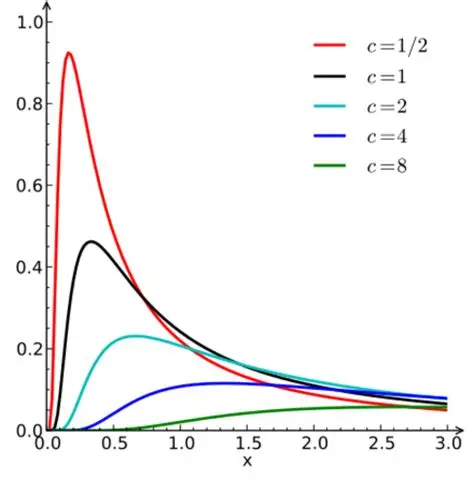
\includegraphics[width=0.75\linewidth]{01_math/03_chapter_calcul_stochastique/levy_dis.png}
    \caption{Lévy PDF}
    \label{fig:placeholder}
\end{figure}


\section{Reflection Principle for Brownian Motion}

\subsection*{Exercice :}

\begin{exerciseBox}[Reflection Principle for Brownian Motion]
Let \( (W_t)_{t \ge 0} \) be a standard Brownian motion and define
\[
M_t := \max_{0 \le s \le t} W_s.
\]

\textbf{Questions:}
\begin{enumerate}
  \item Show that for any \( a > 0 \),
  \[
  \mathbb{P}(M_t \ge a) = 2\,\mathbb{P}(W_t \ge a) = \mathbb{P}(|W_t| \ge a).
  \]
  % \item Show that for any \( a > 0 \) and \( b < a \),
  % \[
  % \mathbb{P}(M_t \ge a,\, W_t \le b) = \mathbb{P}(W_t \ge 2a - b),
  % \]
  % and deduce that
  % \[
  % \mathbb{P}(M_t \ge a \mid W_t = b) = \exp\!\left(-\frac{2(a-b)a}{t}\right)
  % \quad \text{for } b < a.
  % \]
\end{enumerate}
\end{exerciseBox}

\subsection*{Solution :}

\textbf{Question 1 : }

Ona : 

\[
\mathbb{P}(W_t \ge a) =\mathbb{P}(W_t \ge a \mid M_t \ge a)\mathbb{P}(M_t \ge a) + \mathbb{P}(W_t \ge a \mid M_t < a)\mathbb{P}(M_t < a)
\]


or  $\mathbb{P}(W_t \ge a \mid M_t < a) = \mathbb{P}(W_t \ge a \mid \max_{0 \le s \le t} W_s < a) = 0$

donc : 

\[
\mathbb{P}(W_t \ge a) =\mathbb{P}(W_t \ge a \mid M_t \ge a)\mathbb{P}(M_t \ge a)
\]

\subsubsection*{Reflection principle :}

For each sample path \( (W_s)_{0 \le s \le t} \) such that
\[
M_t \ge a \quad \text{and} \quad W_t < a,
\]
define its \emph{reflected path} with respect to level \(a\):
\[
\widetilde{W}_s :=
\begin{cases}
W_s, & s \le \tau_a,\\[3pt]
2a - W_s, & s > \tau_a,
\end{cases}
\qquad
\text{where } \tau_a := \inf\{ s \ge 0 : W_s = a \}.
\]
This reflection keeps the law of the Brownian motion unchanged (since increments are symmetric and independent).

\begin{figure}[h]
    \centering
    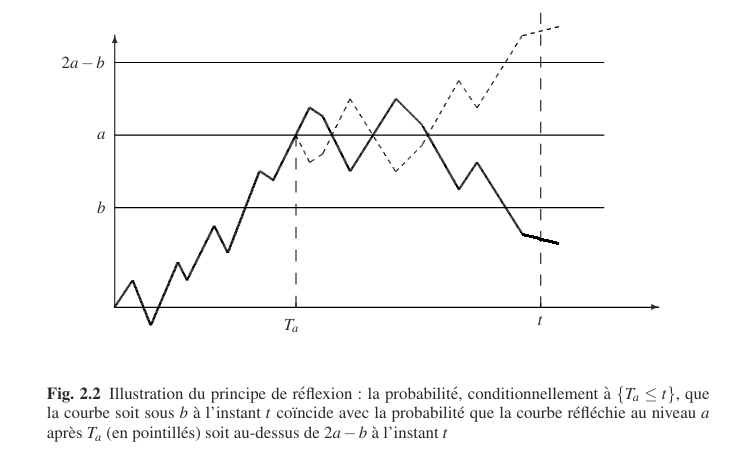
\includegraphics[width=0.75\linewidth]{01_math/03_chapter_calcul_stochastique/reflexion_bm.png}
    \caption{Reflection principle: mapping paths of $W_t$ that hit level $a$ and end below $b$ to reflected paths ending above $2a - b$.}
    \label{fig:placeholder}
\end{figure}


thus : 

\[
\begin{cases}
\mathbb{P}(W_t \ge a \mid M_t \ge a) = \mathbb{P}(W_t < a \mid M_t \ge a) \\
&\\
\mathbb{P}(W_t \ge a \mid M_t \ge a) + \mathbb{P}(W_t < a \mid M_t \ge a) = 1
\end{cases}
\]

so 
\[
\mathbb{P}(W_t \ge a \mid M_t \ge a) = \frac{1}{2}
\]

hence : 

\[
\boxed{
\mathbb{P}(M_t \ge a) = 2\,\mathbb{P}(W_t \ge a) 
}
\]


\textbf{Question 2 : }

For \(b < a\),:

The reflected path maps bijectively the event

\[
\{ M_t \ge a,\, W_t < b \}
\quad \text{to} \quad
\{ W_t > 2a -b  \}.
\]
Hence,

\[
\mathbb{P}(M_t \ge a,\, W_t \le b)
= \mathbb{P}(W_t \ge 2a - b).
\]

Indeed, a path that hits \(a\) before time \(t\) and ends below \(b\)
is mirrored into a path ending above \(2a - b\).


% \textbf{Question 3 : }

% Using the Gaussian law \(W_t \sim \mathcal{N}(0,t)\),
% \[
% \mathbb{P}(M_t \ge a \mid W_t = b)
% = \frac{\mathbb{P}(M_t \ge a, W_t \le b)}{\mathbb{P}(W_t \le b)}
% = \frac{\mathbb{P}(W_t \ge 2a - b)}{\mathbb{P}(W_t \le b)}
% = \frac{\phi\!\left(\frac{2a - b}{\sqrt{t}}\right)}{\phi\!\left(\frac{b}{\sqrt{t}}\right)},
% \]

% where \( \phi(x) = \frac{1}{\sqrt{2\pi}} e^{-x^2/2} \).
% Simplifying the ratio gives:
% \[
% \boxed{
% \mathbb{P}(M_t \ge a \mid W_t = b)
% = \exp\!\left(-\frac{2(a-b)a}{t}\right),
% \quad b < a.
% }
% \]



